\documentclass{jsarticle}
\usepackage[margin = .7in]{geometry}
\usepackage[dvipdfmx]{graphicx}
\usepackage{listings}
\usepackage{amsmath}
\usepackage{amsfonts}
\usepackage{bm}
\usepackage{ascmac}
\usepackage{MnSymbol}
\usepackage{multirow,array}
\usepackage{comment}
\newcommand{\argmin}{\mathop{\rm arg~min}\limits}
\lstset{%
  language={python},
  basicstyle={\small},%
  identifierstyle={\small},%
  commentstyle={\small\itshape},%
  keywordstyle={\small\bfseries},%
  ndkeywordstyle={\small},%
  stringstyle={\small\ttfamily},
  frame={tb},
  breaklines=true,
  columns=[l]{fullflexible},%
  numbers=left,%
  xrightmargin=0zw,%
  xleftmargin=3zw,%
  numberstyle={\scriptsize},%
  stepnumber=1,
  numbersep=1zw,%
  lineskip=-0.5ex%
}

\begin{document}
\title{Empirical Test on Pure Strategy Nash Equilibrium : Entry Game Case}
\author{池上 慧}
\maketitle

\begin{abstract}
	実証研究で広く用いられる完備情報参入ゲームを用いて、実験環境外のデータから現実の企業の意思決定において混合戦略ナッシュ均衡がプレイされているかを統計的に検定する手法を提案する。これはBattle of Sexesにおける混合戦略のように不安定な均衡はプレイされないというゲーム理論の予測について検証する手法であると同時に、多くの場合純粋戦略ナッシュ均衡のプレイを仮定し分析を進める実証産業組織論の基幹部分についてのテストでもある。提案された手法は、スポーツやゲームといった限定的な状況に限らず、利得構造についても統計的に推定しなくてはならない場合においても簡単な特定化のテストでゲーム理論に関する実証研究を行うことができるという点で有益なものである。
\end{abstract}

\section{Introduction}
データの拡充と推定手法の開発、そしてそれを可能にする計算環境の実現に伴い戦略的状況を扱った実証分析は近年大きく進展している分野である。静学ゲームでは例えば\cite{1}で行われた寡占市場の分析や\cite{2},\cite{3},\cite{4}の参入の分析、\cite{5}による社会的相互作用モデルを用いたpeer effectの分析などが戦略的状況を扱った代表的な研究である。また動学ゲームにおいても、\cite{6}で開発された参入退出ゲームと\cite{9}や\cite{10}で開発された推定手法を用いて\cite{7}や\cite{8}などで動学的な要素を考慮した戦略的意思決定の実証が行われている。

こういった戦略的な状況の分析の基盤は現実のデータがある種の均衡状態から生み出されたものであるという構造を仮定することにある。静学ゲームでは完備情報下では純粋戦略ナッシュ均衡、不完備情報下であれば純粋戦略ベイジアンナッシュ均衡がプレイされているとしてモデルのパラメータを推定する。動学ゲームにおいても同様にマルコフ完全均衡がプレイされているという仮定の下でモデルのパラメータを推定する。

しかし現実にはモデルの予測するある種の均衡が必ずしもプレイされるわけではないということが実験を通して明らかにされてきた。そもそもナッシュ均衡の各種精緻化概念も現実をよりよく説明するために生み出されてきたものであるが、ホニャやホゲが提案した認知階層モデルやlevel-kモデルなどの限定合理性モデルも既存の均衡では予測できない実験データを説明するために作られたモデルである。こういったモデルの正当性は実験データをどれだけ説明できるかという基準で検証されるが、それはそのモデル自体の正当性ではなく、他のモデルと比しての妥当性に過ぎない。また、\cite{12}が指摘したようにデータへのフィットという観点でモデルの妥当性を図ることには正当性がない場合も存在する。

このようにモデルや均衡概念自体への検証というトピックは実験データを用いた場合にすら厳密な蓄積が少ないが、現実のデータを用いる場合にはほとんど研究の蓄積がない。\cite{13}はサッカーのペナルティキックにおける混合戦略ナッシュ均衡の実証を行い、\cite{11}はスウェーデンで実際に行われたゲームを用いて実験的状況下にないデータから均衡概念のチェックを行っている。こういった研究においても扱われる事象は極めて限定的かつ特殊なものであり、社会で広く観察される現象に対する均衡概念の検証はほとんど行われていない。この困難は研究者には観測できない変数の存在や異質性の問題、そしてそもそも利得が観測できずそれ自体が推定する対象であるパラメータであるという事実などによると考えられる。

本研究では広く観察される市場参入という現象に対して、戦略的状況の分析で一般に仮定される純粋戦略ナッシュ均衡を仮説検定によって検証する手法を提案する。モデルは\cite{2}で提案された完備情報参入ゲームを用いる。本論は以下のように進む。2章では関連する研究として\cite{11}と\cite{13}をレビューし、均衡に対する検証がなぜ困難かを整理する。3章では主要な結果を述べる。その際にモデルの説明、純粋戦略がとられていない場合の推定手法、純粋戦略ナッシュ均衡への検定という順番で進む。4章では結語としてより包括的な枠組みの可能性を述べる。


\section{Literatures}

\cite{13}はゲーム理論の予測の統計的な検証を実験環境外のデータを用いて行った稀有な研究である。具体的にはサッカーのプロリーグにおけるペナルティキックでキッカーとキーパーのとった行動のデータを用いて、同時手番としてプレイされているかの検証と混合戦略がプレイされているかの検証を行っている。手番の検証は自身の行動を相手の行動に回帰した時の係数の有意性により判断し、混合戦略に関しては実際の得失点を特定の行動に回帰した時の係数の有意性により判断している。結果としては同時手番という仮説は棄却されず、混合戦略をプレイしているという仮説も棄却されなかったため、実験環境外の戦略的状況下で混合戦略ナッシュ均衡がプレイされるということの証拠となった。しかしペナルティキックという限定的な事象に対する実証であることや、ナッシュ均衡が混合戦略でただ一つ存在する単純なゼロサムゲームについての分析であるということから、現実に観察される多様な経済現象を分析できる手法ではない。本論文で扱う参入ゲームは幅広い産業分野実証が重ねられてきた領域であり、利得構造もゼロサムではないより広範な利得構造を表現できる。

\cite{11}はスウェーデンで実際に行われたくじを用いるゲームでの行動データからナッシュ均衡やその他の限定合理的なモデルの予測能力を検証したものである。実施されたのはLUPIと呼ばれるゲームであり、参加者は$1$から$99999$の間から好きな整数を選び、ただ一人にのみ選ばれた数字のうちで最も小さい数字を選んだプレイヤーが勝利者となり賞金を受け取るというゲームであった。筆者はこれを\cite{21},\cite{22}にしたがってポワソンゲームとして定式化し、ポワソンゲームのナッシュ均衡では実際の行動データが説明できないこと、そして限定合理性のモデルである認知階層モデルでは実データの分散をよく説明できることを示した。しかし先にも述べたようにデータへのフィットの良さを裏付けとしてナッシュ均衡をはじめとしたモデルや構造を正当化することには懸念がある。ポワソンゲームにおける均衡は計算で求めることができるため、ナッシュ均衡とのフィットは一定の妥当性を持つことが想定されるが、認知階層モデルやlevel-kといったモデルはその予測がデータと良くフィットするように、パラメータの値や階層の分布、level-0の割合などが様々に特定化されている。これらを考慮した時、ある種のフィットの良さ以外にモデルや特定化のテストをする枠組みがゲームの構造に対しても必要であると考える。

\cite{11}で引用されているRobert Aumannの言葉にある通り、戦略的な状況を記述し分析するためにはそのゲームが厳格なルールを持っている必要がある。特に均衡概念を検証するという目的のためにはこれが重要であり、そのため利得がコントロールされ、均衡での挙動を計算できる\cite{11}のようなゲーム的状況や\cite{13}で扱われたスポーツ、データの集積も盛んで厳密なルールが参加者にも徹底されるオークションなどの限定的な状況しか検証に用いることができない。しかし一般に実証研究の対象となる経済事象はそのような理想的な状況ではなく、情報構造や利得の構造、さらに手番に関しても研究者にとっては不確実なものである。以下で扱う参入ゲームもその例外ではなく、実証に用いられるモデルは様々に特定化されている。

その特定化の一つとして純粋戦略ナッシュ均衡がプレイされているという仮定が置かれる。これは実現した結果についてプレイヤーが両者ともに別の行動をとればよかったと後悔することがないということを意味するが、支配戦略が存在しない場合においては強すぎる仮定である。通常のゲーム理論の文脈では参入ゲームにおける混合戦略ナッシュ均衡は安定でない均衡であるために予測としては用いられないが、実データにおいても何らかの理由で不安定な均衡が排除されているかを検証するという意味においても、純粋戦略ナッシュ均衡がプレイされるという仮定を検証する枠組みを提示することには意義がある。

\section{Model and Equilibrium}
\subsection{Toy Model}
以下の利得表を持つ参入ゲームを考える。
\begin{table}[h]
    \caption{Toy model 利得表}
    \centering
    \setlength{\extrarowheight}{2pt}
    \begin{tabular}{cc|c|c|}
      & \multicolumn{1}{c}{} & \multicolumn{2}{c}{Player $2$}\\
      & \multicolumn{1}{c}{} & \multicolumn{1}{c}{参入しない}  & \multicolumn{1}{c}{参入する} \\\cline{3-4}
      \multirow{2}*{Player $1$}  & 参入しない & $(0,0)$ & $(0,\theta_{\mu}+\epsilon_2)$ \\\cline{3-4}
      & 参入する & $(\theta_{\mu}+\epsilon_1,0)$ & $(\theta_{\mu}+\theta_{\delta}+\epsilon_1, \theta_{\mu}+\theta_{\delta}+\epsilon_2)$ \\\cline{3-4}
    \end{tabular}
\end{table}
ここで、$\theta_{\mu}$は一社のみ参入することができた時に得られ利得であり、$\theta_{\delta}$は二社が参入してしまった時の利得減少分を表すパラメータである。$\theta_{\delta}$は以下で競争効果と呼ぶ。$(\epsilon_1, \epsilon_2)$はプレイヤー同士では観測可能だが研究者には観測できない利得であり、標準正規分布に従うとする。この確率変数は各市場ごとに毎期生成される、つまりデータとして得られる市場ではそれぞれプレイヤーは異なる利得表のゲームをプレイしていることに注意する。以下「参入しない」を$0$、「参入する」を$1$で表記する。

プレイヤーは合理的であるとし、支配戦略がある時はその戦略をとることができるとする。例えばプレイヤー1については、
\begin{align*}
	\begin{cases}
		{\rm Pr}(\text{player 1 takes $0$}) = 1\quad \text{if}\ \epsilon_1 < -\theta_{\mu}\\
		{\rm Pr}(\text{player 1 takes $1$}) = 1\quad \text{if}\ \epsilon_1 > -\theta_{\mu} - \theta_{\delta}
	\end{cases}
\end{align*}
である。

また、支配戦略を用いて行動の逐次削除もできるとする。すなわち、相手にとって支配戦略が存在する時はその事実を用いて自身の行動について被支配戦略を削除することで行動を確定させることができる。例えばプレイヤー1について$-\theta_{\mu} < \epsilon_1 < -\theta_{\mu} - \theta_{\delta}$の時、
\begin{align*}
	\begin{cases}
		{\rm Pr}(\text{player 1 takes $0$}) = 1\quad \text{if}\ \epsilon_2 > -\theta_{\mu} - \theta_{\delta}\\
		{\rm Pr}(\text{player 1 takes $1$}) = 1\quad \text{if}\ \epsilon_2 < -\theta_{\mu}
	\end{cases}
\end{align*}
以上の仮定はSecond Order Rationalityと呼ばれる仮定であり、以降SORと呼称する。SORの下でプレイヤーの行動が確定しないのは$\left\{ (\epsilon_1, \epsilon_2) \mid -\theta_{\mu} < \epsilon_1 < -\theta_{\mu} - \theta_{\delta}\ \wedge\  -\theta_{\mu} < \epsilon_2 < -\theta_{\mu} - \theta_{\delta} \right\}$のみである。この領域(以下$\largestar$)における純粋戦略ナッシュ均衡は$(0,1),\ (1,0)$の二つである。

$\largestar$においては$x$をプレイヤー1の参入しない確率、$y$をプレイヤー2の参入しない確率とした時に$(x, y) = \left( \frac{\theta_{\mu} + \theta_{\delta} + \nu_2}{\theta_{\delta}} ,  \frac{\theta_{\mu} + \theta_{\delta} + \nu_1}{\theta_{\delta}} \right)$が混合戦略ナッシュ均衡として存在する。$\largestar$において混合戦略がプレイされることは$(\epsilon_1, \epsilon_2) \in \largestar$でも一定の確率で$(1,1),\ (0,0)$が実現してしまうことを意味する。よって推定の際にはこの$(1,1),\ (0,0)$が実現する割合の歪みを適切に処理することが必要である。

\subsection{General Model}
上記の単純なモデルを\cite{3}のようにプレイヤーとマーケットの性質によって利得が変化し、競争効果もプレイヤーによって異なる一般のモデルへと拡張する。データは$M$市場について$T$期分得られているとする。市場$m \in \left\{ 1, \cdots, M\right\}$におけるプレイヤー$i \in \left\{ 1,2\right\}$の利得に関わる$K$個の変数をまとめて${\bf x}_{m, i}$の確率ベクトルで表記する。これを用いてプレイヤー$i$の利得$(u_i)$は以下のように欠ける。
\begin{align*}
	u_i = {\bf x}_{m, i}^{'} \beta_i + \delta_i {\bf 1}[y_{-i} = 1]+ \epsilon_i
\end{align*}
ここで${\bf 1}[y_{-i} = 1]$は相手プレイヤーが参入することの指示関数であり、$\delta_i$はプレイヤー$i$の競争効果、$\epsilon_i$は標準正規分布に従う研究者には観測不可能な確率的な効用である。これを用いて市場$m$における利得表は以下のように書くことができる。
\begin{table}[h]
    \caption{general model 利得表}
    \centering
    \setlength{\extrarowheight}{2pt}
    \begin{tabular}{cc|c|c|}
      & \multicolumn{1}{c}{} & \multicolumn{2}{c}{Player $2$}\\
      & \multicolumn{1}{c}{} & \multicolumn{1}{c}{参入しない}  & \multicolumn{1}{c}{参入する} \\\cline{3-4}
      \multirow{2}*{Player $1$}  & 参入しない & $(0,0)$ & $(0,{\bf x}_{m, 2}^{'} \beta_2+\epsilon_2)$ \\\cline{3-4}
      & 参入する & $({\bf x}_{m, 1}^{'} \beta_1+\epsilon_1,0)$ & $({\bf x}_{m, 1}^{'} \beta_1+\delta_1+\epsilon_1,\ {\bf x}_{m, 2}^{'} \beta_2+\delta_2+\epsilon_2)$ \\\cline{3-4}
    \end{tabular}
\end{table}

toy modelと同様にSORの仮定を置くと、市場$m$ごとの$\largestar_m$で$(x, y) = \left( \frac{({\bf x}_{m, 1}^{'} \beta_1 + \delta_1 + \epsilon_2}{\delta_1} ,  \frac{{\bf x}_{m, 2}^{'} \beta_2 + \delta_2 + \epsilon_1}{\delta_2} \right)$を混合戦略ナッシュ均衡として持つ。


\section{Inference}
以下では一般のモデルにおけるパラメータの推定量として、$\largestar_m$における均衡の仮定に応じて3種類与える。一つ目の仮定は純粋戦略ナッシュ均衡の仮定(以下pure strategy Nash equilibriumを略してPNと呼称する)である。すなわち$\largestar_m$においては必ず$(0,1), (1,0)$のどちらかが実現するという仮定の下で推定するものであり、ここでは\cite{2}において考案された複数均衡に対して頑健な参入企業数を結果変数として用いた最尤推定量を紹介する。この推定量を以下PN推定量と呼ぶ。二つ目の仮定は$\largestar_m$においては必ず混合戦略ナッシュ均衡に従ってエームがプレイされるという仮定(以下Always mixed strategy Nash equilibriumを略してAMNと呼称する)である。すなわち$\largestar_m$においてもある確率で$(1,1), (0,0)$がプレイされてしまう状況を想定し、それによって生じる参入企業数の実現確率の歪みを考慮して推定する手法を与える。これによって得られた推定量を以下でAMN推定量と呼ぶ。三つ目は$\largestar_m$において純粋戦略ナッシュ均衡と混合戦略ナッシュ均衡がどのような割合で実現していてもパラメータを一致推定できる頑健な推定量を与える。これを以下ではRobust推定量と呼ぶ。

\subsection{PN推定量}
純粋戦略を仮定した時、$\largestar_m$においては複数の均衡が存在するので単純にプレイヤーの参入結果を結果変数に用いると、すべての事象の実現確率を足すと$1$を超えてしまうため適切な尤度を構成できない。しかし、$\largestar_m$において二つある純粋戦略ナッシュ均衡の結果がどちらも1社のみ参入するという結果であることを利用して、参入した企業の数を結果変数としたBivariate Probitを行うことでパラメータが推定できる。

市場$m$に着目する。$t_2^m$を2社がどちらも参入した回数、$t_0^m$をどちらも参入しなかった回数とする。企業$i$について参入することが支配戦略となる確率と参入しないことが支配戦略となる確率とをそれぞれ$(q_i^1, q_i^0)$で表記する。これは$\phi(\cdot),\ \Phi(\cdot)$をそれぞれ標準正規分布の確率密度関数、確率分布関数とした時以下のように書ける。
\begin{align*}
\begin{cases}
	q_i^1 = \int_{-{\bf x}_{m, i}^{'} \beta_i - \delta_i}^{\infty} \phi(\epsilon_i) \mathrm{d}\epsilon_i = \Phi({\bf x}_{m, i}^{'} \beta_i + \delta_i)\\[10pt]
	q_i^0 = \int_{-\infty}^{-{\bf x}_{m, i}^{'} \beta_i} \phi(\epsilon_i) \mathrm{d}\epsilon_i = \Phi(-{\bf x}_{m, i}^{'} \beta_i)
\end{cases}
\end{align*}

従って市場$m$におけるデータを$D^m$、パラメータの組を$\theta$で表記すると対数尤度は以下のようである。またこれによって得た推定量を$\theta^P$で表記する。
\begin{align*}
	&\sum_{m = 1}^M g(D^m \mid \theta)\\[10pt]
	&\text{where}\quad g(D^m \mid \theta) = t_2^m\ {\rm log} (q_1^1 q_2^1) + t_0^m\ {\rm log} (q_1^0 q_2^0) + (T - t_2^m - t_0^m)\ {\rm log} (1- q_1^1 q_2^1 - q_1^0 q_2^0)
\end{align*}


\subsection{AMN推定量}
\begin{figure}[h]
\centering
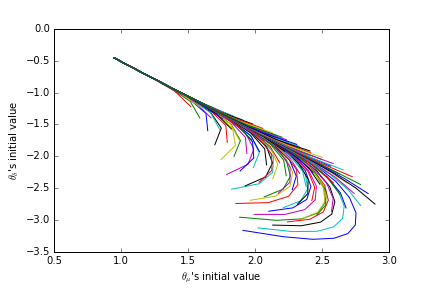
\includegraphics{conversion.png}
\caption{収束の様子}
\end{figure}
$\largestar_m$において混合戦略がプレイされているとした時に、$t_2^m$と$t_0^m$の中でどれだけが混合戦略の結果として実現したものであるかを求める。

ベイズの定理より以下が成立する。ただし二つ目の等式はSORの仮定より成立する。
\begin{align*}
	&{\rm Pr}(\text{(1,1) is NE}\ \mid\ \text{(1,1) is played}) \\[8pt]
	&= \frac{{\rm Pr}(\text{(1,1) is played}\ \mid\ \text{(1,1) is NE})\ {\rm Pr}(\text{(1,1) is NE})}{{\rm Pr}(\text{(1,1) is played}\ \mid\ \text{(1,1) is NE})\ {\rm Pr}(\text{(1,1) is NE}) + {\rm Pr}(\text{(1,1) is played}\ \mid\ \text{(1,1) is not NE})\ {\rm Pr}(\text{(1,1) is not NE})}\\[8pt]
	&= \frac{{\rm Pr}(\text{(1,1) is NE})}{{\rm Pr}(\text{(1,1) is NE}) + {\rm Pr}(\text{(1,1) is played}\ \mid\ \text{(1,1) is not NE})\ {\rm Pr}(\text{(1,1) is not NE})}\\[8pt]
	&= \frac{{\rm Pr}(\text{(1,1) is NE})}{{\rm Pr}(\text{(1,1) is NE}) + {\rm Pr}(\text{(1,1) is played} \wedge \largestar_m)}
\end{align*}
1社も参入しない場合についても同様の計算ができる。ここで修正項は以下のように計算できる。
\begin{align*}
\begin{cases}
	c_2^m = {\rm Pr}(\text{(1,1) is played} \wedge \largestar_m) = \Pi_{i = 1}^2 \left\{ \frac{{\bf x}_{m, i}^{'} \beta_i }{\delta_i} \left( \Phi({\bf x}_{m, i}^{'} \beta_i) - \Phi({\bf x}_{m, i}^{'} \beta_i  + \delta_i) \right) + \frac{1}{\delta_i} \left( \phi({\bf x}_{m, i}^{'} \beta_i ) - \phi({\bf x}_{m, i}^{'} \beta_i  + \delta_i) \right) \right\}\\[10pt]
	c_0^m = {\rm Pr}(\text{(0,0) is played} \wedge \largestar_m) = \Pi_{i = 1}^2 \left\{ \frac{{\bf x}_{m, i}^{'} \beta_i +\delta_i}{\delta_i} \left( \Phi({\bf x}_{m, i}^{'} \beta_i) - \Phi({\bf x}_{m, i}^{'} \beta_i  + \delta_i) \right) + \frac{1}{\delta_i} \left( \phi({\bf x}_{m, i}^{'} \beta_i ) - \phi({\bf x}_{m, i}^{'} \beta_i  + \delta_i) \right) \right\}
\end{cases}
\end{align*}

以上より
\begin{align*}
	f_2^m(\theta) = \frac{q_1^1 q_2^1}{q_1^1 q_2^1+ c_2}\quad\ f_0^m(\theta) = \frac{q_1^0 q_2^0}{q_1^0 q_2^0+ c_0}
\end{align*}
とすれば以下のように対数尤度を構成できる。

\begin{align*}
	&\sum_{m = 1}^M h(D^m \mid \theta)\\[10pt]
	&\text{where}\quad h(D^m \mid \theta) = t_2^m\ f_2^m(\theta)\ {\rm log} (q_1^1 q_2^1) + t_0^m\ f_0^m(\theta)\ {\rm log} (q_1^0 q_2^0) + (T - t_2^m\ f_2^m - t_0^m\ f_0^m)\ {\rm log} (1- q_1^1 q_2^1 - q_1^0 q_2^0)
\end{align*}

Toy modelにおいてAMNのサンプルデータを用いてこの推定を試す。$(\theta_{\mu}, \theta_{\delta}) = (1, -0.5)$を真の値とするときの収束の様子は図1のようであり、正しく収束することがわかる。またこれによって得た推定量を$\theta^M$で表記する。ここで用いたアルゴリズムについてはAppendixに記す。

\subsection{Robust推定量}
\begin{figure}[h]
\centering
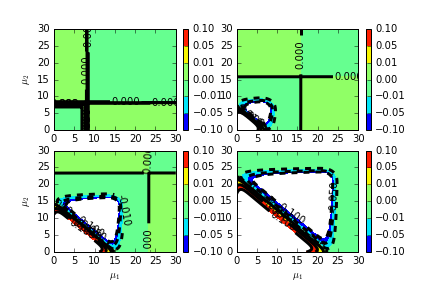
\includegraphics{diff3.png}
\caption{頑健性 左上から順に$\delta = -0.01$, $\delta = -7.4$, $\delta = -15$, $\delta = -22.5$の時の等高線}
\end{figure}

\begin{figure}[h]
\centering
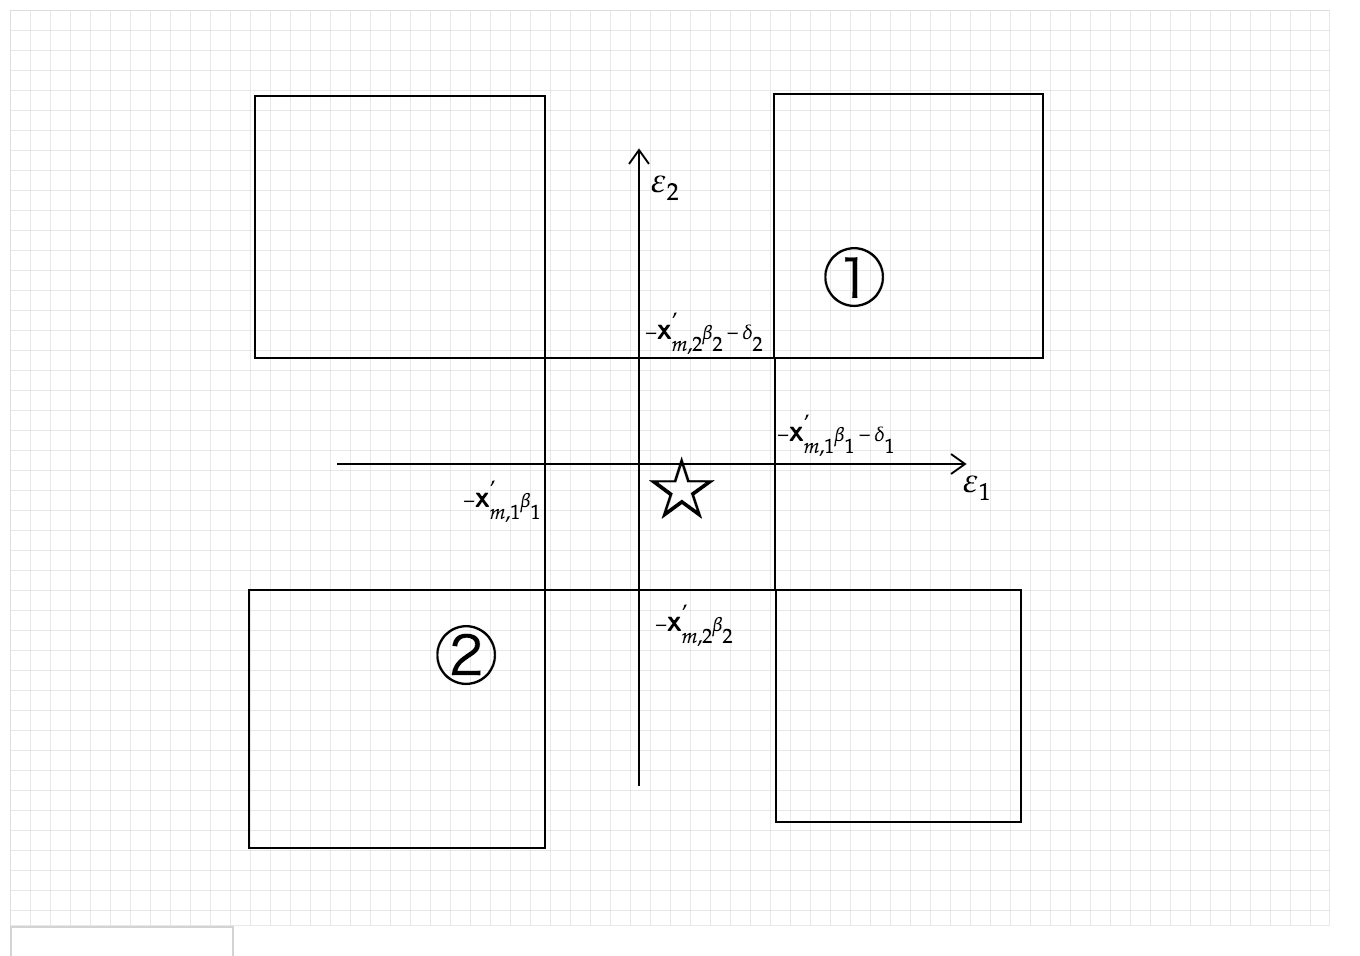
\includegraphics[scale = 0.3]{brgraph.png}
\caption{均衡の分布}
\end{figure}

$\largestar_m$における均衡選択メカニズムとして、$w \in [0,1]$の確率で混合戦略ナッシュ均衡が実現するとする。すなわち先のPNの仮定は$w = 0$を、AMNの設定は$w = 1$の場合を想定していると解釈できる。またこのメカニズムに以下の仮定を置く。

\begin{description}
\item[仮定1:uniform equilibrium selection mechanism] $w$は$(\epsilon_1, \epsilon_2)$に依存しない。
\end{description}

ここで1社も参入しない確率と両者ともに参入する確率との差分を$\alpha(w)$と書くと、
\begin{align*}
	\alpha(w) = w\ \left\{ G_1 G_2 \left( 1 + \frac{{\bf x}_{m, 1}^{'} \beta_1}{\delta_1} + \frac{{\bf x}_{m, 2}^{'} \beta_2}{\delta_2} \right) + \frac{G_1g_2}{\delta_2} + \frac{G_2g_1}{\delta_1} \right\}
\end{align*}
ただし、
\begin{align*}
\begin{cases}
	G_i =  \Phi({\bf x}_{m, i}^{'} \beta_i) - \Phi({\bf x}_{m, i}^{'} \beta_i  + \delta_i)\\
	g_i = \phi({\bf x}_{m, i}^{'} \beta_i) - \phi({\bf x}_{m, i}^{'} \beta_i  + \delta_i)
\end{cases}
\end{align*}
である。

この時以下の二つが成立する。
\begin{description}
	\item[主張1] $\left| \alpha(w) \right|$は$w$についての増加関数である。
	\item[主張2] $\forall i \in \left\{ 1,2\right\}$で${\bf x}_{m, i}^{'} \beta_i + \delta_i$が十分に大きいならば$\alpha(1)$を十分0に近づけることができる。
\end{description}

主張1は$w$を固定した時、$\left| \alpha(w) \right| = w\left| c_0 - c_2 \right|$とかくことができるため明らかである。主張2については図2より確認できる。図2は$\mu_i = {\bf x}_{m, i}^{'} \beta_i$として、$\delta = \delta_1 = \delta_2$という対称性の仮定の下で各$(\mu_1, \mu_2, \delta)$に対して$\alpha(1)$の値を出力し、$\delta$の値ごとに等高線で表示したものである。

図2からわかるように$\mu_i + \delta$が両プレイヤーにとって十分大きい領域では$\alpha(1)$が十分小さくなっている。すなわちパラメータにこの性質を満たすという仮定を課せば、PNとAMNのどちらの仮定の下でも1社も参入しない確率と両者ともに参入する確率との差分は図3の\textcircled{\scriptsize 2}と\textcircled{\scriptsize 1}の領域の差分に収束することを意味する。また、図示のためにおいた$\delta_i$についての対称性の仮定を緩めてもこれは同じように成立する。

さらに主張1より$\alpha(1)$が十分0に近い領域のパラメータセットにおいては他のいかなる$w \in [0,1]$においても十分0に近いことがわかる。従って「$\forall i \in \left\{ 1,2\right\}$で${\bf x}_{m, i}^{'} \beta_i + \delta_i$が十分に大きい」という仮定の下では、$\largestar_m$においていかなる均衡選択メカニズムが存在しようと、「1社も参入しない確率と両者ともに参入する確率との差分は図3の\textcircled{\scriptsize 2}と\textcircled{\scriptsize 1}の領域の差分に収束する」というモーメント条件を用いてパラメータの推定を行うことができる。

以上の議論よりRobust推定量$(\theta^R)$は以下のように定義される。
\begin{align*}
	&\theta^R = \argmin_{\theta} \sum_{m = 1}^M r(\hat{p^m} ; \theta)^2\\[10pt]
	&\text{where}\ r(\hat{p^m} ; \theta) = (\hat{p_2^m} - \hat{p_1^m}) - (q_1^1 q_2^1 - q_1^0 q_2^0)
\end{align*}

識別に関しては以下が成立する。
\begin{description}
	\item[主張3] \cite{3}の除外制約の下でRobust推定量$(\theta^R)$は識別可能である。
\end{description}
証明はAppendixに記す。


\section{Hypothesis Test}
前章で述べた頑健な推定量を用いてハウスマン検定により純粋戦略ナッシュ均衡の仮定に対する仮説検定を行うことを考える。ただし、通常のハウスマン検定では有効推定量を用いるのに対し、\cite{3}で述べられたようにPN推定量は有効推定量ではない。従って非有効推定量どうしを用いたハウスマン検定を考える必要があることに注意する。

\subsection{PNのtest}
パラメータの真の値を$\theta^0$で表記すると先の3つの推定量について漸近分布は以下で与えられる。
\begin{align*}
	\begin{pmatrix}
	\sqrt{M}(\theta^P - \theta^0)\\[8pt]
	\sqrt{M}(\theta^M - \theta^0)\\[8pt]
	\sqrt{M}(\theta^R - \theta^0)
	\end{pmatrix}\ \xrightarrow{d}\ 
	N\left( \begin{pmatrix}0\\[8pt]0\\[8pt]0
	\end{pmatrix},\ 
	\begin{pmatrix}
	A_{11} & A_{12} & A_{13}\\[8pt]
	A_{21} & A_{22} & A_{23}\\[8pt]
	A_{31} & A_{32} & A_{33}
	\end{pmatrix}
	\right)
\end{align*}

ここで$r(\theta) = \frac{1}{M} \sum_m r(\hat{p^m} ; \theta)$として$R(\theta) = \frac{\mathrm{d}r}{\mathrm{d} \theta^{'}}$とする。このとき、以下の二つの行列を用いることで漸近分散を$A S A^{'}$と表すことができる。
\begin{align*}
	S = Var\begin{pmatrix}
	\frac{1}{\sqrt{M}} \sum_m \nabla_{\theta} g(D^m \mid \theta^0)\\[8pt]
	\frac{1}{\sqrt{M}} \sum_m \nabla_{\theta} h(D^m \mid \theta^0)\\[8pt]
	\frac{1}{\sqrt{M}} \sum_m\ r(p^m \mid \theta^0)
	\end{pmatrix},\ 
	A = \begin{pmatrix}
	-E\left[ \nabla_{\theta \theta^{'}}g(D^m \mid \theta^0) \right]^{-1} & 0 & 0\\[8pt]
	0 & -E\left[ \nabla_{\theta \theta^{'}}h(D^m \mid \theta^0) \right]^{-1} & 0\\[8pt]
	0 & 0 & -\left( R(\theta^0)^{'} R(\theta^0) \right)^{-1} R(\theta^0)^{'}
	\end{pmatrix}
\end{align*}

ここで純粋戦略ナッシュ均衡に対するハウスマン検定統計量$H_1$は$q_1 = \sqrt{M} (\theta^P - \theta^R)$と置いたとき以下で定義される。
\begin{align*}
H_1 = q_1^{'} \left( \hat{Avar\left( q_1 \right)} \right)^{-1} q_1
\end{align*}
ただし$\hat{Avar\left( q_1 \right)}$は$q_1$の分散共分散行列の推定値であり、デルタメソッドから以下で求められる。
\begin{align*}
	\hat{Avar\left( q_1 \right)} = \hat{A_{11}} - \hat{A_{13}} - \hat{A_{31}} + \hat{A_{33}} 
\end{align*}
ここで$\left(\hat{A_{11}},\ \hat{A_{13}},\ \hat{A_{31}},\ \hat{A_{33}} \right)$は各要素のサンプルからの推定値である。帰無仮説は「$\largestar_m$で純粋戦略ナッシュ均衡が常に実現する」であり、帰無仮説の下で$H_1$は自由度$2K + 2$の$\chi^2$分布に従う。これを利用し有意水準$5\%$の仮説検定を行うことができる。

\subsection{AMNのtest}
同様の枠組みで帰無仮説をAMNとしたときのハウスマン検定統計量$(H_2)$は以下のように構成できる。ただし$q_2 = \sqrt{M}\left( \theta^M - \theta^0 \right)$である。
\begin{align*}
	&H_2 = q_2^{'} \left( \hat{Avar\left( q_2 \right)} \right)^{-1} q_2\\[10pt]
	&\text{where}\ \hat{Avar\left( q_2 \right)} = \hat{A_{22}} - \hat{A_{23}} - \hat{A_{32}} + \hat{A_{33}} 
\end{align*}
帰無仮説の下で$H_2$は自由度$2K + 2$の$\chi^2$分布に従うので、有意水準$5\%$の仮説検定を行うことができる。

\section{Conclusion}
本論文では広く用いられる完備情報参入ゲームのモデルを用い、実データにおいて純粋戦略ナッシュ均衡がプレイされているかを統計的に検定できる簡便な手法を提案した。先行研究ではスポーツやゲームなどの限定的な状況でのみ均衡に関する実証研究が行われていたが、参入ゲームというより広く観察でき、複雑な利得構造を持つ現象についてもプレイされる均衡を統計的にテストできる枠組みを提示したことが本論文の主要な貢献である。これはまた、ゲーム理論の文脈では不安定な均衡として排除される混合戦略ナッシュ均衡の存在を実データを用いて検証することができるため、均衡の精緻化という観点でも有益な示唆を与えるであろう。

\subsection{Further Research}
上記の推定量はすべて$M$市場に関して$T$期分の2社についての参入結果がデータとして得られている理想的な状況を想定した。しかし、\cite{15}で扱われるような企業参入に関するデータは$M$市場について1回の参入結果がデータとして得られている場合が多い。また、仮に$M$市場についてそれぞれ複数期の参入結果が得られたとしても、研究者には観測不可能な効用が各回で独立に発生するケースは想定しにくい。すなわち、同じ市場について複数かいの参入結果が得られているのであれば、その結果は系列相関を持つはずであり、上記のように同じ市場について十分な分散を保証してくれる可能性は低い。

従って上記のフレームワークを実際に用いるためには$ M$市場について一回だけ参入結果が得られているようなデータセットについても実行できるように修正をする必要がある。このためには\cite{4}のような不完備情報の参入ゲームと同様に1段階目で各市場における参入企業数の予測値をノンパラメトリックに推定し、それを用いて2段階目で構造パラメータを推定する手法をとることができる。しかし、不完備情報参入ゲームで必要とされたのが各企業の均衡における参入確率であるのに対して完備情報ゲームで上記のRobust推定量を得るためには各市場における両者が参入する確率とどちらも参入しない確率とをそれぞれ指定し、さらにその差を用いることになる。そのため多量のサンプルが必要とされることに注意する必要がある。

また、\cite{15}のように実際に完備情報ゲームとして寡占市場とそこにおける競争効果を分析した文献ではプレイヤーが2人ではないケースが扱われることにも注意が必要である。\cite{15}ではアメリカにおける航空輸送産業が例として扱われているが、日本においてもコンビニエンスストアや低価格飲食チェーン店などの商業立地においては2社による競争よりも複数企業間での競争が多く観察されることは疑いなく、またそれにより企業ごとに異なる競争効果を細かく分析することは当該産業における立地などの規制に関する政策評価を行う際に重要な要素となる。従ってプレイヤーが2社以上存在する市場においても上記の検定を拡張する必要がある。

本論文においてはナッシュ均衡という構造を前提とし、さらに情報構造についても完備情報であるという仮定の下で、均衡の種類の特定化についての検定を提示した。混合戦略が現実にプレイされているかというゲーム理論の実証研究という観点でこれは重要なものであるが、実証産業組織論においてより有益な分析を行っていくためには、より基幹となる仮定であるナッシュ均衡という構造自体や情報構造についての検証を行っていくことも同様に肝心である。実際、\cite{16}や\cite{17}などでは実際のスーパーマーケットの立地データを用いて情報構造についての検定が行われており、より柔軟な情報構造に頑健な均衡概念を用いた分析も行われている。また、ナッシュ均衡という構造自体に対して仮定を緩めることを試みる研究も存在する。例えば\cite{18}では完備情報ゲームにおいて合理性の仮定を緩めた際の識別集合を様々なモデルについて報告している。さらに\cite{19},\cite{20}では様々な均衡概念を実データを用いて検定する手法が開発されている。

これらの均衡概念の検証も未だ静学ゲームが主であり、動学参入退出のモデルや価格付けのモデルなど広いクラスの問題を扱うことのできる検定手法の開発が今後望まれる研究の方向性である。そのためには特定化やパラメータの仮定を最小限に抑えるデータドリブンな手法が望ましい方向性であると考える。

\section{Appendix}
\subsection{AMN推定量の推定アルゴリズム}
図1を出力する際に用いた推定アルゴリズムを以下に記す。$4.2$で述べた通り本来は$f_2^m(\theta), f_0^m(\theta)$を含め最尤法で推定できるが、微分が煩雑となるためここでは
\lstinputlisting[caption=逐次推定アルゴリズム]{AMN.py}

\subsection{主張3の証明}
\begin{align*}
	&\theta^R = \argmin_{\theta} \sum_{m = 1}^M r(\hat{p^m} ; \theta)^2\\[10pt]
	&\text{where}\ r(\hat{p^m} ; \theta) = (\hat{p_2^m} - \hat{p_1^m}) - (q_1^1 q_2^1 - q_1^0 q_2^0)
\end{align*}
について\cite{3}と同様の除外制約の下で点識別可能であることを示す。

プレイヤー2の利得のみ動かす変数が存在する時、${\bf x}_{m, 2}^{'} \beta_2\ \to \infty$となる領域が存在する。この時$-{\bf x}_{m, 2}^{'} \beta_2\ \to -\infty$であることから以下が成立する。
\begin{align*}
\begin{cases}
	q_1^1 q_2^1 - q_1^0 q_2^0\ \to \Phi({\bf x}_{m, 1}^{'} \beta_1 + \delta_1)\ \text{where}\ {\bf x}_{m, 2}^{'} \beta_2\ \to \infty\\[10pt]
	q_1^1 q_2^1 - q_1^0 q_2^0\ \to -\Phi({\bf x}_{m, 1}^{'} \beta_1)\ \text{where}\ {\bf x}_{m, 2}^{'} \beta_2\ \to -\infty
\end{cases}
\end{align*}
これはプレイヤー2の行動がプレイヤー1の行動によらずに定るケースであり、プレイヤー1についても同様に考えることができるので、$E\left[ {\bf x}_{m, i} {\bf x}_{m, i}^{'} \right]$が$i = \left\{ 1,2 \right\}$についてどちらも逆行列が存在するならば$\theta$は識別可能である。

\section{References}
\begin{thebibliography}{10}
	\bibitem{1} Bresnahan/寡占
	\bibitem{2} Bresnahan and Reiss
	\bibitem{3} Tamer 2003
	\bibitem{4} Seim 2006
	\bibitem{5} Brock and Durlauf
	\bibitem{6} Pakes and McGuire
	\bibitem{7} Collard and Wexler 2013
	\bibitem{8} Ryan 2012
	\bibitem{9} BBL 2007
	\bibitem{10} AM 2007
	\bibitem{11} Ostring et al 2011
	\bibitem{12} Haile 2008
	\bibitem{13} Levitt サッカー
	\bibitem{14} Eric van Damme 1998
	\bibitem{15} Ciliberto and Tamer 
	\bibitem{16} Grieco
	\bibitem{17} Magnolfi and Roncoroni 2017
	\bibitem{18} Aradillas-Lopez and Tamer 2008
	\bibitem{19} Kashaev 2017 a
	\bibitem{20} Kashaev 2017 b
	\bibitem{21} Myerson 1998
	\bibitem{22} Myerson 2000
\end{thebibliography}


\end{document}
























